\documentclass[10 pt,usenames,dvipsnames, oneside]{article}
\usepackage{../../../modelo-ensino-medio}



\begin{document}

\begin{center}
  \begin{minipage}[l]{3cm}

\includegraphics[width=2cm]{logo}    
\end{minipage}\hfill
\begin{minipage}[r]{.8\textwidth}
 {\Large \scshape Atividade: }  
\end{minipage}
\end{center}
\vspace{.2cm}

\ifdefined\prof
%Habilidades da BNCC
\begin{objetivos}
\item \textbf{EM13MAT316} Resolver e elaborar problemas, em diferentes contextos, que envolvem cálculo e
interpretação das medidas de tendência central (média, moda, mediana) e das de dispersão
(amplitude, variância e desvio padrão).
\item \textbf{EM13MAT408} Construir e interpretar tabelas e gráficos de frequências, com base em dados obtidos em pesquisas por amostras estatísticas, incluindo ou não o uso de softwares que interrelacionem estatística, geometria e álgebra.
\end{objetivos}

%Caixa do Para o Professor
\begin{goals}
%Objetivos específicos
\begin{enumerate}
\item Determinar a média, mediana e variância, a partir de um histograma.
\end{enumerate}

\tcblower

%Orientações e sugestões
Esta atividade pretende mostrar a utilidade das fórmulas apresentadas nesta seção para obter medidas de posição e dispersão, quando não se conhecem os dados separadamente.
\end{goals}

\bigskip
\begin{center}
{\large \scshape Atividade}
\end{center}
\fi

Os resultados obtidos na prova de seleção para vagas de estágio numa empresa estão representados no histograma a seguir.
\phantomsection\label{\detokenize{PE104-A:fig-hist-vagas-estagio}}
\begin{figure}[H]
\centering

\noindent\includegraphics[width=.25\linewidth]{{exercicio9}.png}
\caption{Histograma das notas na prova de seleção para vagas de estágio}
\label{\detokenize{PE104-A:fig-hist-vagas-estagio}}\end{figure}

\begin{enumerate}
\item {} 
Com base neste histograma, calcule a média, a variância, a mediana, a moda, o primeiro quartil e o terceiro quartil.

\item {} 
Usando a informação do histograma, faça um esboço do boxplot destes dados.

\end{enumerate}

\ifdefined\prof
\begin{solucao}

\begin{enumerate}
\item A média pode ser calculada por 
\begin{align*}
\bar{x}&\approx0{,}15\cdot1+0{,}25\cdot3+0{,}20\cdot5+0{,}3\cdot7+0{,}1\cdot9\\
&=0{,}15+0{,}75+1+2{,}1+0{,}9=4{,}9.
\end{align*}

Para calcular a variância, primeiro obtemos uma aproximação para a soma de quadrados das notas, dada por
\begin{align*}
&0{,}15\cdot12+0{,}25\cdot32+0{,}20\cdot52+0{,}3\cdot72+0{,}1\cdot92=\\
&0{,}15+2{,}25+5+14{,}7+8{,}1=30{,}2, 
\end{align*}
assim, $s^2\approx30{,}2−4{,}92=6{,}19$.

A classe modal corresponde ao intervalo delimitado por $6$ e $8$, uma aproximação para o valor modal é considerar o ponto médio da classe modal. Neste caso, temos que $7$ é uma aproximação para o valor da moda nesta distribuição.

Não podemos identificar quem é o valor central ou valores centrais, pois não foi dada a informação do número de candidatos que fizeram a prova. Mas isso não é problema, pois a mediana divide a distribuição em dois intervalos de frequências iguais a $50\%$. Logo, precisamos identificar em que intervalo, cairá a mediana e, como apresentado na Organizando as ideias: medidas de posição tomar o ponto médio desta classe como aproximação para o valor da mediana. Observe na figura que a frequência do primeiro intervalo é $0{,}15$; a frequência acumulada, considerando os dois primeiros intervalos é $0{,}15+0{,}25=0{,}40$ ainda é menor do que $0{,}5$. Considerando os três primeiros intervalos, a frequência acumulada é $0{,}4+0{,}2=0{,}6$. Logo, a mediana está no intervalo delimitado por $4$ e $6$, de modo que tomamos o ponto médio deste intervalo como uma aproxmação para o valor da mediana, a saber, $5$.

O mesmo raciocínio utilizado para obter a mediana, pode ser usado para obter aproximações do primeiro e terceiro quartis. Em vez de $50\%$ na frequência acumulada, deveremos encontrar $25\%$ e $75\%$, respectivamente. Como a frequência do primeiro intervalo é $0{,}15$ e a frequência acumulada, considerando os dois primeiros intervalos é $0{,}15+0{,}25=0{,}40$, seque que o primeiro quartil deve estar no segundo intervalo delimitado por $2$ e $4$. Logo, tomamos o ponto médio deste intervalo como uma aproximação para o primeiro quartil, a saber, 3. Até o terceiro intervalo a frequência acumumulada é $0{,}6$, considerando o quarto intervalo, a frequência acumulada é $0{,}9$. Logo, como o terceiro quartil está no quarto intervalo, tomamos o ponto médio $7$ com aproximação para o terceiro quartil.

\item Com base no histograma temos o seguinte esquema dos cinco números $Min=0$, $Q_1=3$, $\text{Mediana}=5$, $Q_3=7$, $\text{Max}=10$. $\text{DQ}=7-3=4$. $\text{Cerca inferior}=3-6=-3$, $\text{cerca superior}=7+6=13$. Logo, não existem valores discrepantes. A figura a seguir ilustra um boxplot para este esquema dos cinco números.
\begin{figure}[H]
\centering

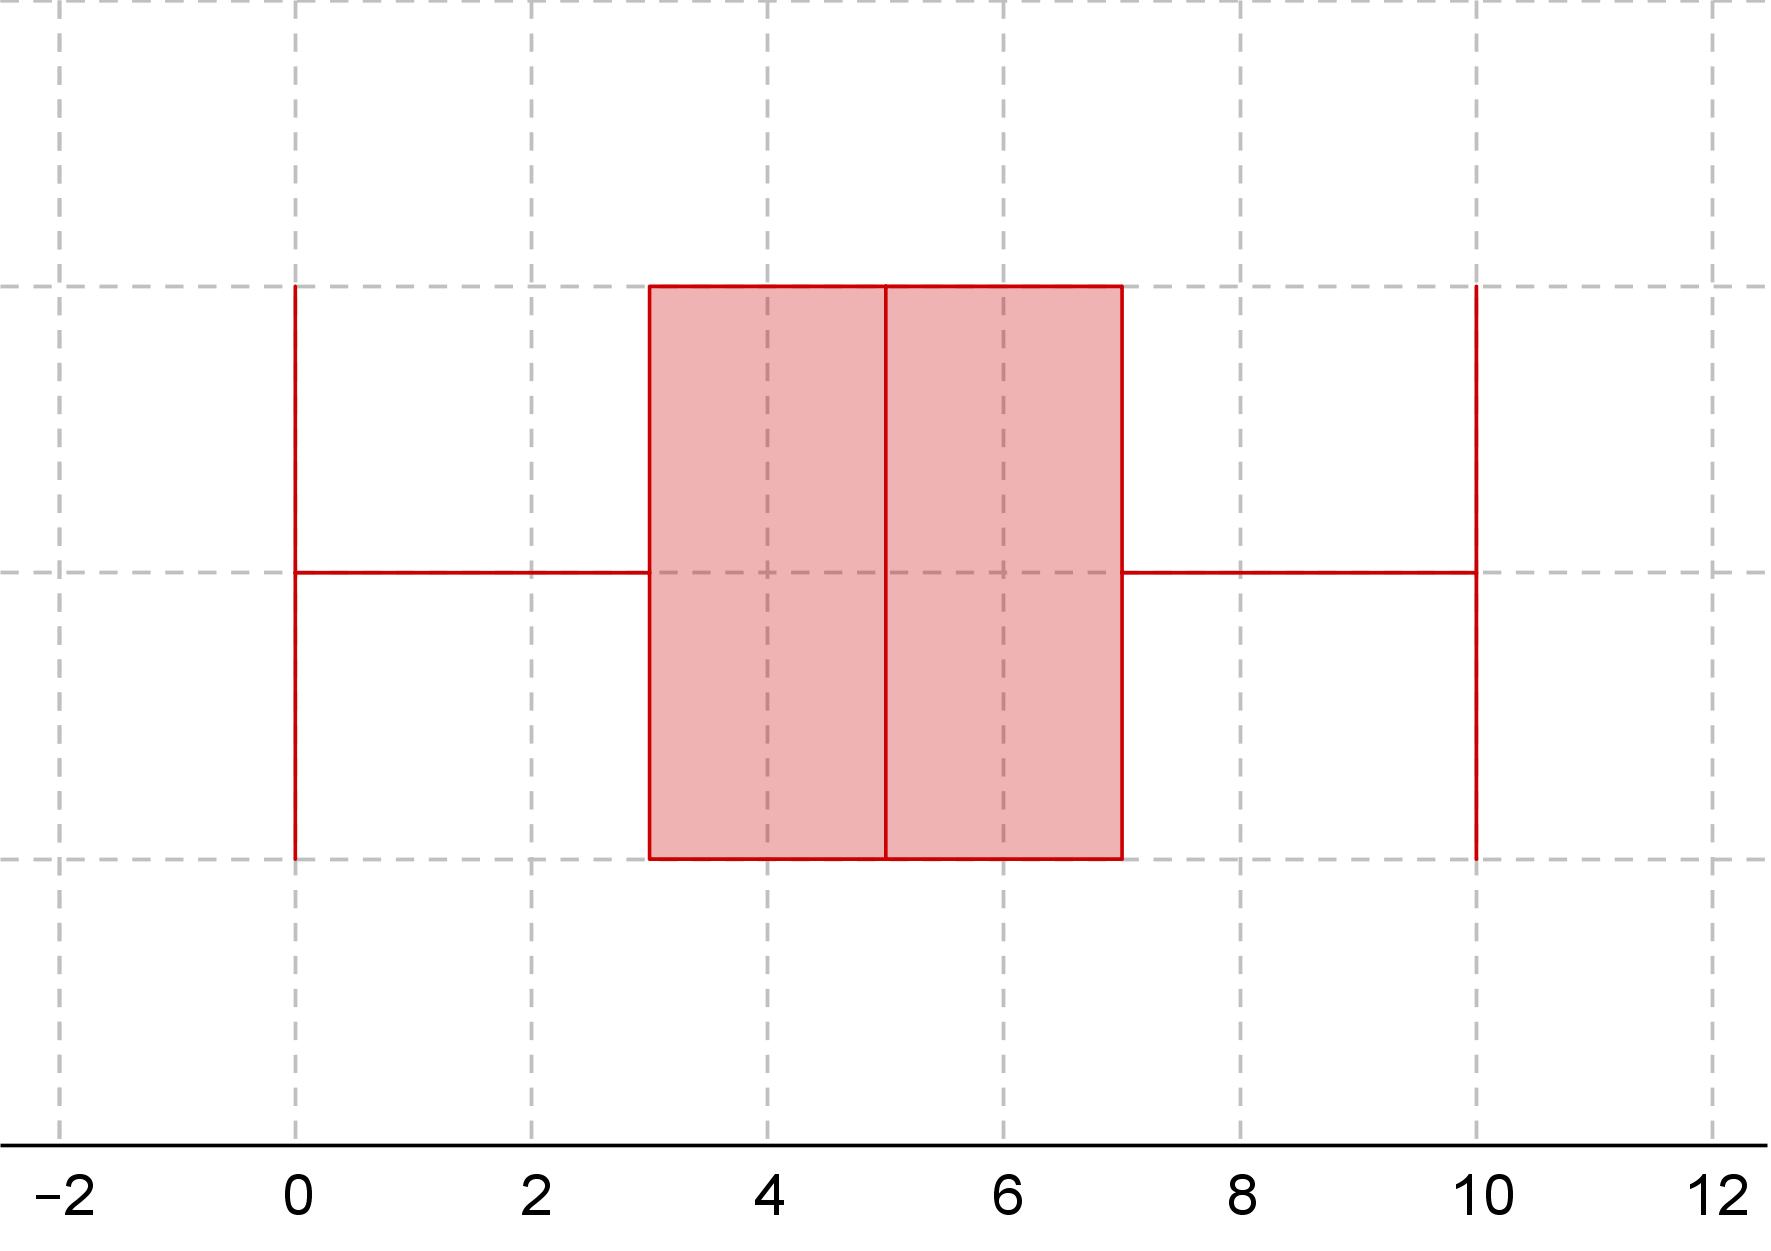
\includegraphics[width=.5\linewidth]{boxplotexercicio9.png}
\caption{Boxplot dos resultados dos candidatos na prova de seleção}
\label{}
\end{figure}
\end{enumerate}

\end{solucao}
\fi

\end{document}